\fancychapter{Experimental Results}
\label{cap:ER}


\section{Experimental Results}
\label{sec:results}

In order to evaluate the performance of the developed system, several tests, with different goals, were developed and executed. First and foremost, the optimization algorithms are tested in order to evaluate their overall quality on a set of benchmark tests. This is followed by a set of tests over the Data Management System, in order to estimate the necessary time to collect the required data to answer to any given request. Finally, the overall utility of the proposed and developed system is evaluated, by performing a series of tests on the Flying Tourist Problem, and comparing the solutions provided by the metaheuristic to those from \textit{random} optimization algorithm, and the nearest neighbor heuristic.

This experiments were executed on a 2.6GHz Intel i7-6700, and all the code was developed using the Python programming language. 

%%__________________________________________________________________
%%_______________________ metaheuristic test _______________________
%%__________________________________________________________________
\subsection{Optimization system}
Given that there are no benchmark tests available for the time-dependent TSP, we tested the algorithms on the classical Traveling salesman. This was followed by a set of tests on TDTSP instances, created by the method described in (\cite{TDTSP_construction}), which uses dual-theory on the Integer Linear formulation for the TDTSP, to generate TDTSP instances whose optimal solution is defined a-priori.

In order to test the performance of the optimization system, 5 set of problems were solved, ranging from 17 to 323 nodes, each problem was executed 5 times, and its results averaged. Note that each algorithm was allowed to run for a maximum of 60 seconds. The choice of executing the metaheuristic for a limited amount of time, instead of a fixed number of iterations, arises from the necessity to produce time-efficient responses to the user. The results of the execution of these tests are presented in table \ref{tab:tsp_results} and \ref{tab:tdtsp_results}, for the asymmetric TSP and time-dependent TSP, respectively.

The analysis of table \ref{tab:tsp_results}, regarding the resolution of TSP benchmark problems, gives some interesting information. For small instances (17 nodes), both ACO and SA present the optimal solution, consistently. For medium instances (35-53 nodes), both algorithm perform in the range of 5-20$\%$ relative error. As for bigger problems ( 170-323 nodes), the performance of the ACO decreases only slightly (22-25\%), while that of the SA becomes much worse (29-63\%). 

The performance of the Simulated Annealing on the test problem $ftv170$, which appears to be somewhat abnormal, due to its very high error, was further analyzed. The tests were repeated 2 more times, averaging the result of 5 execution, for a total duration of 60 seconds each. The quality of the results did not improve. So, instead of running the algorithm for just 60 seconds, we executed a series of tests were it run for a longer time, 180 seconds. This time, the results were somewhat better, presenting a relative error of 45.72\%, as opposed to the previous 63\%. While this improvement is still low from the desirable amount, it suggest that, with enough time, the Simulated Annealing could possible present much better solutions.

Looking now at the performance over the time-dependent TSP, presented in table \ref{tab:tdtsp_results}, the results are very different from thus of the classic TSP. First of all, no optimal solution could be consistently found. Furthermore, the relative error was only above 10\% once, and this occurs for the smallest instance (p17), using the ACO algorithm. (This suggests that the algorithm is stuck, using to much heuristic information, and low exploration. Given that the heuristic parameter $\beta$, is very high, this is not surprising. The confirmation of this is given by the better performance on the bigger instances.)

The comparison of the SA vs the ACO deserves some extra notes. First of all, it is worth nothing that, at each iteration of both algorithms, the same number of solutions are created, since the markov chain length, and the number of ants, are both set to $N$, the number of nodes. A comparison of the number of iterations executed by each algorithm, over the 60 available seconds, leads to the conclusion that SA performs much more iterations than the ACO. This should come as no surprise, given that the SA relies on local search and improvement heuristic, while ACO requires the \textit{construction} of solutions. This for itself is not the problem. The problem is that the solution construction process of the ACO is somewhat complex and computational heavy. At each ant construction step, several difficult calculations have to be performed, as to select the following solution component. 

Despite being heavier and slower, the Ant Colony System appears to be, overall, slightly better than the Simulated Annealing, even without the use of local search procedures. Another advantage of the Ant Colony Optimization is that good solutions are produced very early, and not only in the late stages of the algorithm execution, as occurs with the Simulated Annealing. This means that an early interruption in the execution of the ACO may still produce good results, while in the Simulated Annealing this becomes very unlikely. 

% Please add the following required packages to your document preamble:
% \usepackage{multirow}
\begin{table*}[t]
\centering
\caption{Performance of the metaheuristics on the \textbf{Asymmetric TSP}.}
\label{tab:tsp_results}
\begin{tabular}{|l|l|l|l|l|l|}
\hline
algorithm            & problem & opt cost & meta cost & num. iterations & rel. error \\ \hline
\multirow{5}{*}{SA}  & br17    & 39       & 39        & 264319.4        & 0          \\ \cline{2-6} 
                     & ftv35   & 1473     & 1641      & 63659           & 11.41      \\ \cline{2-6} 
                     & ft53    & 6905     & 7963      & 36189.2         & 15.32      \\ \cline{2-6} 
                     & ftv170  & 2755     & 4486.4    & 6714.4          & 62.84     \\ \cline{2-6} 
                     & rbg323  & 1326     & 1706.2    & 1361.8          & 28.67      \\ \hline
\multirow{5}{*}{ACO} & br17    & 39       & 39        & 6892.7          & 0          \\ \cline{2-6} 
                     & ftv35   & 1473     & 1552.4    & 1469.6          & 5.39       \\ \cline{2-6} 
                     & ft53    & 6905     & 8269.6    & 689.2           & 19.76      \\ \cline{2-6} 
                     & ftv170  & 2755     & 3359.4    & 67.8            & 21.93      \\ \cline{2-6} 
                     & rbg323  & 1326     & 1660.4    & 19.6            & 25.21      \\ \hline
\end{tabular}
\end{table*}


% Please add the following required packages to your document preamble:
% \usepackage{multirow}
\begin{table*}[]
\centering
\caption{Performance of the optimization algorithm on the \textbf{time-dependent TSP}.}
\label{tab:tdtsp_results}
\begin{tabular}{|l|l|l|l|l|l|}
\hline
algorithm            & problem & opt cost & meta cost & num. iterations & rel. error \\ \hline
\multirow{5}{*}{SA}  & p17     & 2458     & 2631.2    & 219517.2        & 7.04       \\ \cline{2-6} 
                     & p35     & 5131     & 5406.8    & 80262           & 5.38       \\ \cline{2-6} 
                     & p53     & 7930     & 8265.6    & 37450.6         & 4.23       \\ \cline{2-6} 
                     & p170    & 25483    & 26427     & 3521            & 3.70       \\ \cline{2-6} 
                     & p323    & 48991    & 51926.8   & 900.6           & 5.99       \\ \hline
\multirow{5}{*}{ACO} & p17     & 2458     & 2729      & 9720.6          & 11.03      \\ \cline{2-6} 
                     & p35     & 5131     & 5500.2    & 2590.6          & 7.20       \\ \cline{2-6} 
                     & p53     & 7930     & 8370.4    & 1099.6          & 5.53       \\ \cline{2-6} 
                     & p170    & 25483    & 26402.4   & 71.2            & 3.61       \\ \cline{2-6} 
                     & p323    & 48991    & 50261.4   & 13.4            & 2.59       \\ \hline
\end{tabular}
\end{table*}




%%__________________________________________________________________
%%_______________________ utility test _____________________________
%%__________________________________________________________________
\subsection{Utility Test}

In order to establish the actual utility of the proposed system, the following experiment was executed. A series of Flying Tourist Problem (FTP) instances were constructed, ranging from just 1 city to visit (which corresponds to a round flight - if the return node is equal to the start node), up to a total of 20 cities. For each problem instance, solutions were constructed using three different algorithms: the random algorithm (explained in the introduction of section \ref{sec:optimization}); the nearest neighbor heuristic; and both ACO and SA metaheuristics. 

For every different instance size, 5 different FTP were considered, and the results averaged. In all cases, the trip starts and returns to Lisbon, and visits a given set of cities, chosen randomly, belonging to (Miami, Moscow, JFK, Hong Kong, Sidney, Dubai, Kiev, Barcelona, Madrid, Dublin, Los Angeles, Beijing, San Francisco, Singapore, Johannesburg, Cairo, Casablanca, Abuja, Frankfurt, Atlanta, Istanbul, Oslo). The start date was always the same, set to \textit{1 July 2018}, which, upon the execution of the tests, was a date 45 days into the future. Finally, the waiting period on \textit{each} city was set to a random value between 1 and 12 days. 

The results provided by the different algorithms are presented in table \ref{tab:utility_0}, and include a comparison of the flight cost and flight duration provided by the different algorithms. Note that $R$ refers to the random algorithm, while $NN$ to the nearest neighbor, and $MC$ and $ME$ to the metaheuristics, utilizing the cost (eq. \ref{eq:obj_cost}) and entropy (eq. \ref{eq:obj_entropy}) objective functions, respectively. This table also presents the completion time of each of these algorithms. 

Note that the nearest neighbor and metaheuristics run only after the complete weight matrix is available, which occurs only once the communication with the third-party API is finished. Note also that, after the weight matrix is complete, the nearest neighbor is run first, followed by the metaheuristic for the cost, and finally by the metaheuristic for the entropy. Thus, the completion time of the nearest neighbor, gives a good estimation, or "upper bound", on the time spent communicating with the third-party API, as to obtain the necessary flight data. Figure \ref{fig:kiwi_response_time} presents an accurate illustration of the time spent communicating with the third-party API, as a function of the number of nodes, and the length of the start-period.  

\begin{figure}[tbp]
  \centering
  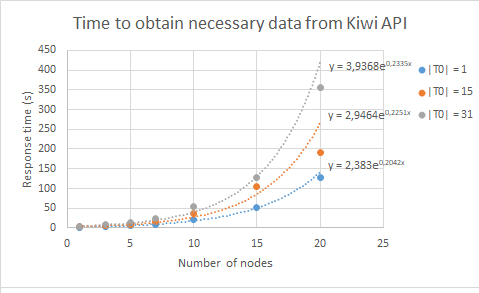
\includegraphics[width=9cm, height=5cm]{./imgs/kiwi_response_time.png}
  \caption{Time spent communication with the Kiwi API, as to obtain the necessary flight data, as a function of the number of nodes, and length of the start-period.}
  \label{fig:kiwi_response_time}  
\end{figure}

As to simplify the comprehension of the results presented in table \ref{tab:utility_0}, figure \ref{fig:prices_0} illustrates the improvement of the total flight cost, for the NN and metaheuristic algorithms, relative to the cost of the initial \textit{random} solution. It is worth noting that, for a single node (round flight), the initial random solution, the nearest neighbor, and the metaheuristic, all produce the same result. For 3 nodes, the nearest neighbor does not present relevant improvement, while the metaheuristic already distances itself, presenting around 5\% improvement. For 5 nodes, this difference increases to 20\%, and at 10 nodes it reaches the 50\% mark. Instances with more nodes, 15-20, continue to improve, slowly, up to 60\%.

\begin{figure}[tbp]
  \centering
  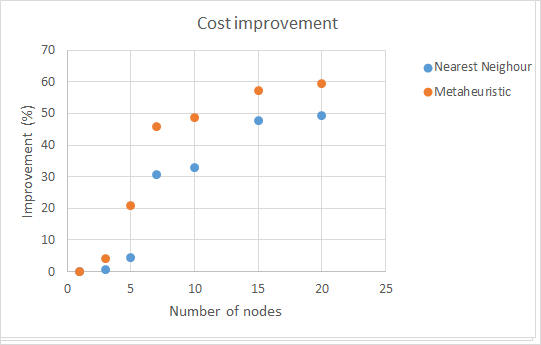
\includegraphics[width=9cm, height=5cm]{./imgs/improvement_0.png}
  \caption{Comparison of the solution cost, of the nearest neighbor and metaheuristic, relative to the initial solution produced, for a single start date.}
  \label{fig:prices_0}  
\end{figure}


\begin{figure}[tbp]
  \centering
  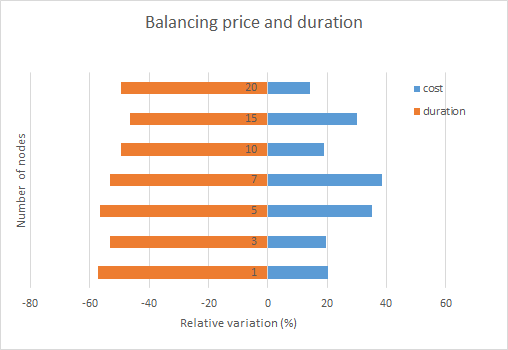
\includegraphics[width=9cm, height=5cm]{./imgs/cost_vs_time.png}
  \caption{Comparison of the variation of the total flight cost and duration, for two different objective functions, minimizing the total cost and entropy.}
  \label{fig:cost_vs_time}  
\end{figure}

We also analyzed the impact of using different objective functions in the optimization process. Instead of optimizing for the total trip cost, the algorithm was set to minimize the entropy, that is, the weighted summation of the flight cost and flight duration. The entropy is set such that the cost weight contributes with 70\%, and the flight duration with the remaining 30\%. After executing the metaheuristic for both objective functions, the total flight cost and duration are compared. The results are illustrated in figure \ref{fig:cost_vs_time}. The inspection of this figure leads to the conclusion that, in general, by increasing the cost by around 20\%, the flight duration decreases to approximately half.


This series of experiments is completed with the execution of the same problems, this time with a start-period of 31 days. The impact in the solution improvement, relative to the trip cost, can be verified in figure \ref{fig:prices_31}. The analysis of this figure leads to the conclusion that, the selection of an extended start-period, as opposed to a single date, leads to a higher increase in the total savings. For the round flight, the improvement of the metaheuristic is around 10\%. This is because the random and the nearest neighbor solution consider a single start date for the solution construction process. Other small instances, with 3 and 5 nodes, present much higher improvements than those with a single start date, ranging from 20-40\%, as opposed to just 5-20\%. For bigger problem instances, the effect of increasing the start-period is less significant, but it exists, providing an improvement of up to 65\%.

\begin{figure}[tbp]
  \centering
  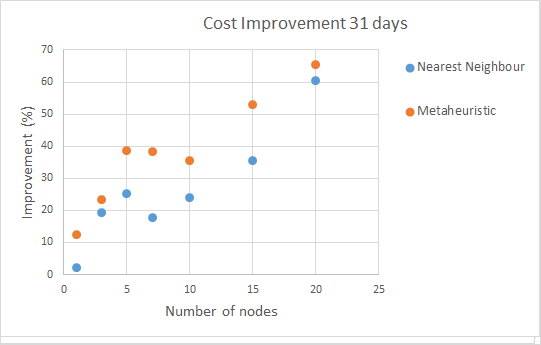
\includegraphics[width=9cm, height=5cm]{./imgs/improvement_31.png}
  \caption{Comparison of the solution cost, of the nearest neighbor and metaheuristic, relative to the initial solution produced, for a start-period of 31 days.}
  \label{fig:prices_31}  
\end{figure}





\begin{table*}[]
  \centering
  \caption{Comparison of the flight cost, flight duration, and execution time, for Flying Tourist Problem instances, ranging from 1 to 20 nodes, for a single start date, using three different algorithms.}
  \label{tab:utility_0}
  \resizebox{\textwidth}{!}{
    \begin{tabular}{|l|l|l|l|l|l|l|l|l|l|l|l|l|}
    \hline
    |N|        & \multicolumn{4}{l|}{Cost (Euro)}  & \multicolumn{4}{l|}{Fly duration (hours)} & \multicolumn{4}{l|}{Completion time (seconds)} \\ \hline
              & R      & NN     & MC     & ME     & R        & NN       & MC       & ME       & R        & NN         & MC         & ME        \\ \hline
    1          & 838.2  & 838.2  & 838.2  & 1158.4 & 82.11    & 82.11    & 82.11    & 37.37    & 2.57     & 5.03       & 7.87       & 12.13     \\ \hline
    3          & 1520.6 & 1512.8 & 1457.8 & 1828.4 & 124.91   & 117.65   & 111.3    & 58.49    & 2.64     & 7.24       & 11.79      & 17.39     \\ \hline
    5          & 2088.6 & 1993   & 1654.8 & 2123.7 & 194.00   & 157.14   & 157.14   & 63.39    & 3.17     & 10.05      & 15.00      & 21.20     \\ \hline
    7          & 3571.2 & 2479   & 1927.6 & 2520.6 & 267.53   & 203.16   & 180.59   & 90.35    & 3.43     & 13.48      & 18.48      & 25.16     \\ \hline
    10         & 4819   & 3228.8 & 2468.2 & 3211.8 & 377.95   & 255.89   & 236.82   & 105.06   & 3.69     & 25.72      & 30.73      & 38.31     \\ \hline
    15         & 7288.8 & 3808.2 & 3103.8 & 3996.6 & 518.21   & 312.66   & 259.83   & 141.81   & 4.59     & 55.33      & 60.37      & 68.91     \\ \hline
    20         & 9187.6 & 4664.6 & 3721.4 & 4704.2 & 665.85   & 343.57   & 324.62   & 162.71   & 5.38     & 133.62     & 138.66     & 148.67    \\ \hline
    \end{tabular}
  }
\end{table*}



























